% v4 Results part B: what the states reconstruct, and the dimension axis
% (register R5-R9). Probe-dilution control (R7) accompanies the dimension
% figure per the locked rule. All numbers through the macros pipeline.

\subsection{What the states reconstruct, and how small they can be}
\label{sec:res_reconstruction}

Decoding closes the loop on the construction story: the same division of
labour that the probes read appears in the decoded fields, scored on
the \TestSplit{} set through identical-capacity frozen decoders with the Wang SSIM
convention of \S\ref{sec:methods_protocol}. With the lift anchor present,
the near-body head buys the same near-body structural fidelity as the wake
head (\TcSsimNbCLN{} for the \LiftState{} against \TcSsimNbCLW{} for the
\PredState), the
collapsed no-$L$ cells sit far below (from \TcSsimNbCW{} for CW), and the
reconstructive anchors reach parity (\TcSsimNbAeLW{} for AE-LW), as an
objective trained on the field should
(figures~\ref{fig:decode} and the per-cell bars in the data record). The
decode panels make the same point qualitatively: all three healthy states
recover the near-body vortex system and the coherent wake at matched
fidelity, and the residual rows concentrate on the fine-grain shed
structures no $32$-coefficient state carries.

The dimension axis splits into two tiers, and the split is the paper's
compression statement (figure~\ref{fig:dimrace}a). At $d = 4$ the
predictive families read the peak loads through a linear probe at
\PoneLowdJepa{} (\PredState{} lineage) and \PoneLowdAero{} (coupled-objective
arm) against \PoneLowdFukami{} for the reconstructive baseline, three
seeds each with non-overlapping ranges; the \LiftState{} lineage trained through
the \DirectFC{} is close to dimension-insensitive on the peaks, from
\LadRexpredDFour{} at $d = 4$ to \PoneRexpredPeak{} at $d = 32$ (three
seeds at both ends), where the \PredState{} lineage declines with $d$ (from
\LadClwDFour{} to \LadClwDThirtyTwo). A four-coefficient lift-critical
state is therefore viable. The wake state is not compressible to it: the
decoded structural fidelity of the same lineage rises monotonically with
dimension (full-frame SSIM \SsimLadFullDFour{} to \SsimLadFullDThirtyTwo,
near-body \SsimLadNbDFour{} to \SsimLadNbDThirtyTwo), so the wake-bearing
state needs $d \geq 16$ while the lift saturates by $d \approx 4$ to $8$.

The probe-dilution control disciplines how the first tier may be read
(figure~\ref{fig:dimrace}b). A multilayer probe nearly equalises every
dimension (from \PdMlpDFour{} at $d = 4$ to \PdMlpDThirtyTwo{} at
$d = 32$ on the \TestSplit{} set): the lift information in the state is
dimension-invariant, and small states do not know more. What changes with
dimension is linear accessibility. The best four coordinates of a larger
state recover only \PdBestFourDEight{} to \PdBestFourDThirtyTwo{} through
a linear read-out, so the code is distributed rather than diluted, and the
$d = 4$ advantage is exactly that four coordinates are what a linear
probe, a filter gain, or a controller reads directly. The honest form of
the two-tier claim is therefore: compact and linear at $d = 4$,
distributed and partly nonlinear above.

\begin{figure}
  \centering
  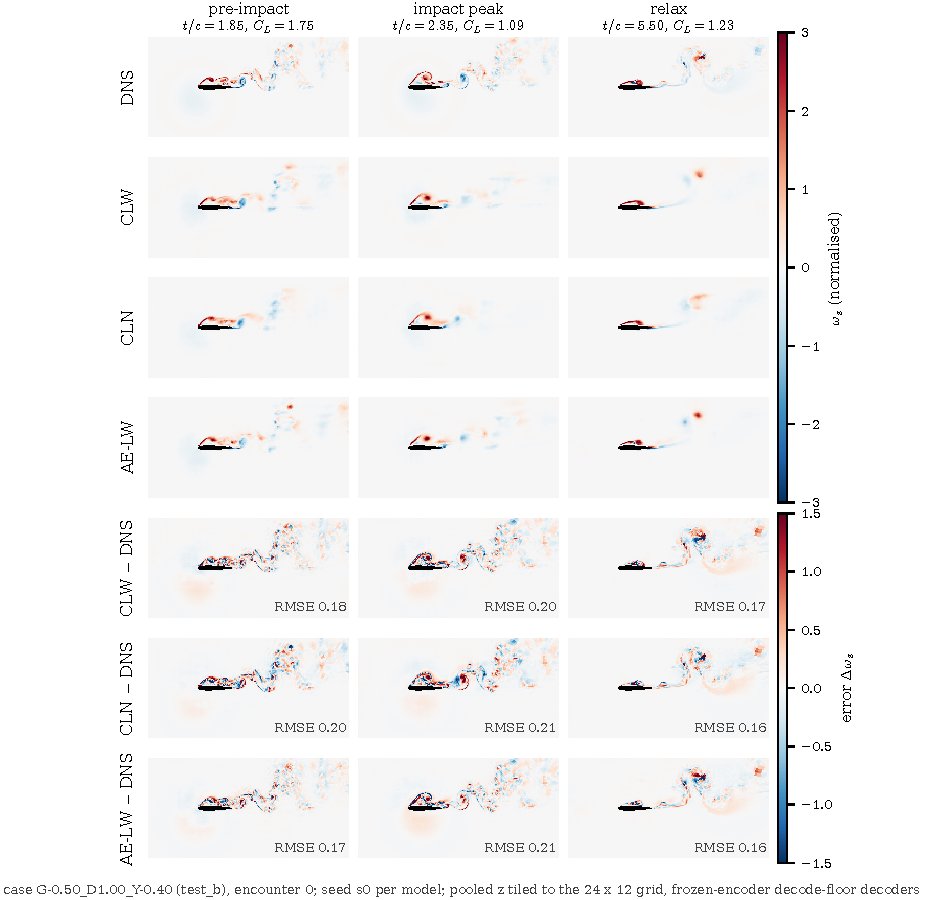
\includegraphics[width=\linewidth]{sections/figures/results/fig_decode_panels_v4.pdf}
  \caption{Decode floor on the representative \TestSplit{} encounter
  (case G$-0.50$\_D$1.00$\_Y$-0.40$, encounter 0; one decoder seed per
  model): DNS, the three healthy states, and the error rows at three
  phases. Identical-capacity frozen decoders; normalised vorticity at the
  fixed $\pm 3$ range.}
  \label{fig:decode}
\end{figure}

\begin{figure}
  \centering
  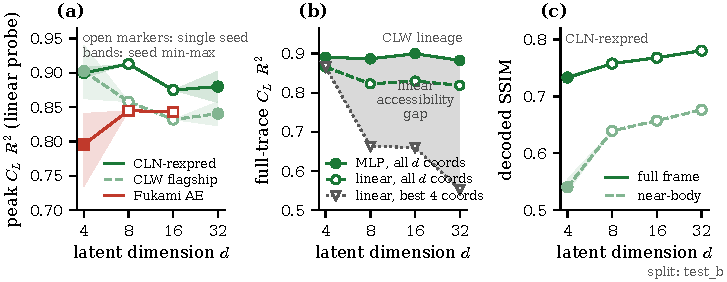
\includegraphics[width=\linewidth]{sections/figures/results/fig_dimension_race_v4.pdf}
  \caption{The dimension axis on the \TestSplit{} set. (a)~Peak-region lift $R^2$
  (linear probe) against latent dimension for the three lineages; shaded
  bands are three-seed min-max ranges, open markers single seeds.
  (b)~The probe-dilution control: a multilayer probe is flat in $d$ while
  the best-four-coordinate linear probe falls, so the $d = 4$ advantage is
  linear accessibility of a distributed code, not information.
  (c)~Decoded SSIM (Wang convention, \S\ref{sec:methods_protocol}) of the
  same lineage rises with $d$: the wake tier is not compressible.}
  \label{fig:dimrace}
\end{figure}
